%%%% Paramétrage du TD %%%%
\def\xxactivite{Révisions \ifprof -- Corrigé \else \fi} % \normalsize \vspace{-.4cm}
\def\xxauteur{\textsl{Xavier Pessoles}}


\def\xxnumchapitre{Révisio  \vspace{.2cm}}
\def\xxchapitre{\hspace{.12cm} Résolution des problèmes de cinématique -- Cinématique du contact ponctuel}
\def\xxonglet{\textsf{Rév -- Cin}}
\def\xxactivite{TD 01}
\def\xxauteur{\textsl{Renan Bonnard}}

\def\xxpied{%
Révision cinématique -- Résolution des problèmes de cinématique\\
Fiche 1 -- \xxactivite%
}

\def\xxcompetences{%
\textsl{%
\textbf{Savoirs et compétences :}\\
%\vspace{-.4cm}
%\begin{itemize}[label=\ding{112},font=\color{ocre}] 
%%\item \textit{Res1.C4 : } Correction
% \item \textit{Res1.C4.SF1 : } Proposer la démarche de réglage d’un correcteur proportionnel
%%proportionnel intégral 
%%et à avance de phase
%\item \textit{Con.C2 : } 	Correction d’un système asservi	
%\item \textit{Con.C2.SF1 : } Choisir un type de correcteur adapté
%\end{itemize}
}}

\def\xxauteur{\textsl{Renan Bonnard}}

\def\xxtitreexo{Roulement à billes}
\def\xxsourceexo{\hspace{.2cm} \footnotesize{}}

\def\xxfigures{
%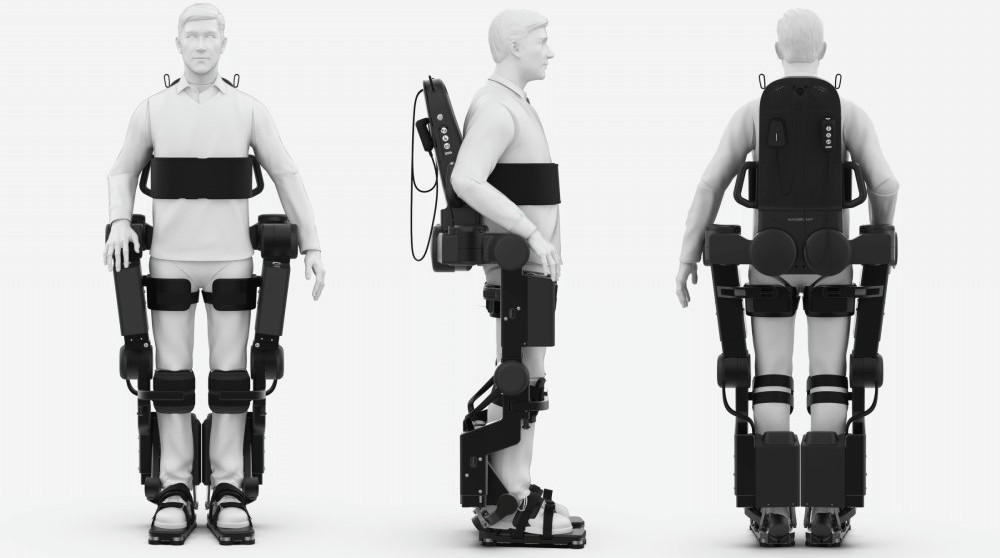
\includegraphics[width=.55\textwidth]{fig_00}
}%figues de la page de garde

\input{\repStyle/pagegarde_TD.tex}
\vspace{4cm}


\ifprof
\else
\begin{multicols}{2}
\fi


\ifprof
\else
Un roulement mécanique est un élément technologique permettant le positionnement, la transmission des efforts et la rotation entre deux pièces par roulement. Ce composant mécanique interposé entre les deux pièces optimise le frottement et la précision de la liaison. Un roulement à billes se présente sous la forme de deux bagues coaxiales entre lesquelles sont placées des billes maintenues espacées par une cage. La fonction de la cage est donc de maintenir deux billes consécutives à distance égale l'une de l'autre lors du fonctionnement du roulement mais elle entraîne aussi des effets nuisibles car il existe un phénomène de glissement entre la cage et les billes. \textbf {L'objectif est d'étudier ce phénomène de glissement.}

\begin{center}
 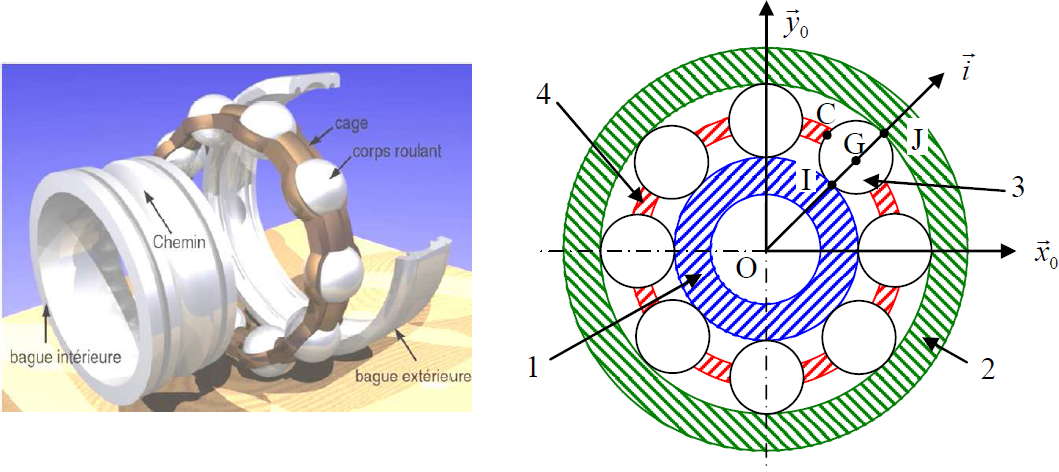
\includegraphics[width=\linewidth]{roulement}
\end{center}


On désigne par :
\begin{itemize}
\item $\mathcal{R}_0 = \left(O,\vect{x_0},\vect{y_0},\vect{z_0}\right)$ le repère associé au bâti 0;
\item $\mathcal{R}_1 = \left(O,\vect{x_1},\vect{y_1},\vect{z_0}\right)$ le repère associé à la bague intérieure 1 en liaison pivot d'axe $(O,\vect{z_0})$ avec le bâti 0 tel que $\theta_1 = \left(\vect{x_0},\vect{x_1}\right) = \left(\vect{y_0},\vect{y_1}\right)$;
\item $\mathcal{R}_2 = \left(O,\vect{x_2},\vect{y_2},\vect{z_0}\right)$ le repère associé à la bague extérieure 2 en liaison pivot d'axe $(O,\vect{z_0})$ avec le bâti 0 tel que $\theta_2 = \left(\vect{x_0},\vect{x_2}\right) = \left(\vect{y_0},\vect{y_2}\right)$;
\item $\mathcal{R}_3 = \left(G,\vect{x_3},\vect{y_3},\vect{z_0}\right)$ le repère associé à la bille 3 qui roule sans glisser sur 1 en I et sur 2 en J et dont on peut considérer qu'elle est en liaison pivot d'axe $(G,\vect{z_0})$ avec la cage 4 tel que $\theta_3 = \left(\vect{x_0},\vect{x_3}\right) = \left(\vect{y_0},\vect{y_3}\right)$;
\item $\mathcal{R}_4 = \left(O,\vect{x_4},\vect{y_4},\vect{z_0}\right)$ le repère associé à la cage 4 en mouvement de rotation autour de $(O,\vect{z_0})$ tel que $\theta_4 = \left(\vect{x_0},\vect{x_4}\right) = \left(\vect{y_0},\vect{y_4}\right)$.
\end{itemize}

Pour faciliter les calculs on définit le repère $\mathcal{R}=\left(O,\vect{i},\vect{j},\vect{z_0} \right)$ tel que, à tout instant, le vecteur $\vect{i}$ possède la même direction et le même sens que le vecteur $\vect{OG}$. Ce repère n'est lié à aucun solide en particulier et ne sert qu'à exprimer simplement les différents termes cinématiques évoqué dans l'énoncé. On pose :

$$
\omega_k = \dot{\theta}_k \quad (k=1,2,3,4) \quad \vect{OI}=r_1 \vect{i} \quad \vect{OJ}=r_2\vect{i} $$
$$
\vect{GC}=\dfrac{1}{2}(r_2-r_1)\vect{j}
$$

\fi

\question{Réaliser les figures planes correspondant au paramétrage du système.}

\question{Déterminer $\vecto{1}{0}$,  $\vectv{O}{1}{0}$ et $\vectv{I}{1}{0}$.}

\ifprof
\begin{corrige}
$$
\left\{ \mathcal{V}(1/0)\right\}=
\left\{
\begin{array}{l}
\vect{\Omega(1/0)}= \dot{\theta}_1 \vect{z_0}\\
\vect{V(O,1/0)}= \vect{0}
\end{array}
\right\}_O
=
\left\{
\begin{array}{l}
\vect{\Omega(1/0)}= \dot{\theta}_1 \vect{z_0}\\
\vect{V(I,1/0)}= r_1 \omega_1 \vect{j}
\end{array}
\right\}_I
$$

\end{corrige} \else \fi



\question{Déterminer $\vecto{2}{0}$,  $\vectv{O}{2}{0}$ et $\vectv{J}{2}{0}$.}

\ifprof
\begin{corrige}
$$
\left\{ \mathcal{V}(1/0)\right\}=
\left\{
\begin{array}{l}
\vect{\Omega(2/0)}= \dot{\theta}_2 \vect{z_0}\\
\vect{V(O,2/0)}= \vect{0}
\end{array}
\right\}_O
=
\left\{
\begin{array}{l}
\vect{\Omega(2/0)}= \dot{\theta}_2 \vect{z_0}\\
\vect{V(J,2/0)}= r_1 \omega_2 \vect{j}
\end{array}
\right\}_J
$$
\end{corrige} \else \fi

\question{Exprimer les conditions de roulement sans glissement en $I$ et $J$. Établir les expression des vecteurs $\vect{V(I,3/0)}$ et $\vect{V(J,3/0)}$.}




\ifprof
\begin{corrige}

$$
\vect{V(I,3/1)}= \vect{0}
$$
$$
\vect{V(I,3/0)}=\vect{V(I,3/1)}+\vect{V(I,1/0)} \Longrightarrow \vect{V(I,3/0)}=\vect{V(I,1/0)} = r_1\omega_1\vect{j}
$$

$$
\vect{V(J,3/2)}= \vect{0}
$$
$$
\vect{V(J,3/0)}=\vect{V(J,3/2)}+\vect{V(J,2/0)} \Longrightarrow \vect{V(J,3/0)}=\vect{V(J,2/0)} = r_2\omega_2\vect{j}
$$

\end{corrige} \else \fi

\question{En déduire l'expression de $\omega_3$ en fonction de $r_1$, $r_2$, $\omega_1$, $\omega_2$.}
\ifprof
\begin{corrige}

$$
\vect{V(I,3/0)}= \vect{V(J,3/0)}+\vect{IJ}\wedge\vect{\Omega(3/0)}
$$
$$
\omega_3 = \dfrac{r_2\omega_2-r_1\omega_1}{r_2-r_1}
$$
\end{corrige}

 \else \fi
%
%\end{multicols}
%\end{document}

\question{Déterminer $\vect{V(G,3/0)}$ en fonction de $r_1$, $r_2$, $\omega_1$, $\omega_2$.}
\ifprof
\begin{corrige}

$$
\vect{V(G,3/0)}= \vect{V(I,3/0)}+\vect{GI}\wedge\vect{\Omega(3/0)} = \dfrac{r_2\omega_2+r_1\omega_1}{2}\vect{j}
$$

\end{corrige} \else \fi


\question{Déterminer l'expression de la vitesse de glissement de la bille 3 par rapport à la cage 4 au point $C$ en fonction de $r_1$, $r_2$, $\omega_1$, $\omega_2$.}

\ifprof
\begin{corrige}

On cherche à calculer $\vect{V(C,3/4)}$ :

$$
\vect{V(C,3/4)}= \vect{V(G,3/4)}+\vect{CG}\wedge\vect{\Omega(3/4)}
$$

Calcul de $\vect{CG}$ :
$$
\vect{CG}=-\dfrac{1}{2}(r_2-r_1)\vect{j}
$$

Calcul de $\vect{\Omega(3/4)}$ :
$$
\vect{\Omega(3/4)}=\vect{\Omega(3/0)}-\vect{\Omega(4/0)}
$$

Calcul de $\omega_4$ :
$$
\vect{V(G,3/4)}=\vect{V(G,3/0)}-\vect{V(G,4/0)}=\vect{0}
$$

Calcul de $\vect{V(G,4/0)}$ :
$$
\vect{V(G,4/0)}=\vect{V(O,4/0)}+\vect{GO}\wedge \vect{\Omega(4/0)}=\dfrac{r_2+r_1}{2}\omega_4\vect{j}
$$

Au final calcul de $\omega_4$ :
$$
\omega_4 = \dfrac{r_2\omega_2+r_1\omega_1}{r_1+r_2}
$$

Calcul de $\vect{\Omega(3/4)}$ : 
$$
\vect{\Omega(3/4)}=\vect{\Omega(3/0)}-\vect{\Omega(4/0)} = \left( \dfrac{r_2\omega_2 -r_1\omega_1}{r_2-r_1} - \dfrac{r_2\omega_2 +r_1\omega_1}{r_2+r_1} \right) \vect{z_0}
$$

Au final en faisant le calcul on obtient : 
$$
\vect{V(C,3/4)} = \dfrac{r_2r_1(\omega_1-\omega_2)}{r_1+r_2}\vect{i}
$$
\end{corrige} \else \fi


\ifprof
\else
\end{multicols}
\fi



